\section{PROVABGS SED Modeling} \label{sec:provabgs}
% brief explanation of the PROVABGS SED modeling 
For each BGS galaxy, we derive its $M_*$ and other properties, 
$\overline{\rm SFR}$, $Z_{\rm MW}$, and $t_{\rm age, MW}$ from DESI
photometry and spectroscopy using the PROVABGS SED modeling
framework~\citep{hahn2022}.  
PROVABGS models galaxy SEDs using stellar population synthesis with
non-parametric star-formation history (SFH) with a starburst, a non-parametric
metallicity history (ZH) that varies with time, and a flexible dust
attenuation prescription.
The non-parameteric SFH and ZH prescriptions are derived from SFHs and ZHs of
simulated galaxies in the Illustris hydrodynamic
simulation~\citep{vogelsberger2014, genel2014, nelson2015} and provide compact 
and flexibly representations of SFHs and ZHs.
For the stellar population synthesis, PROVABGS uses the Flexible Stellar
Population Synthesis~\citep[FSPS;][]{conroy2009, conroy2010b} model with MIST
isochrones~\citep{paxton2011, paxton2013, paxton2015, choi2016, dotter2016},
\cite{chabrier2003} initial mass function (IMF), and a combination of
MILES~\citep{sanchez-blazquez2006} and BaSeL~\citep{lejeune1997, lejeune1998,
westera2002} spectral libraries.

Furthermore, PROVABGS provides a Bayesian inference framework that infers
full posterior probability distributions of the SED model parameter:
$p(\theta\given {\bf X}^{\rm photo}, {\bf X}^{\rm spec})$, where 
${\bf X}^{\rm photo}$ represents the photometry and ${\bf X}^{\rm spec}$ 
represents the spectroscopy. 
In total, $\theta$ has 13 parameters: $M_*$, 6 parameters specifying the SFH
($\beta_1, \beta_2, \beta_3, \beta_4, f_{\rm burst}, t_{\rm burst}$), 2
parameters specifying ZH ($\gamma_1, \gamma_2$), 3 parameters specifying
dust attenuation ($\tau_{\rm BC}, \tau_{\rm ISM}, n_{\rm dust}$), and a
nuisance parameter for the fiber aperture effect. 
Posteriors have distinct advantages over point estimates because they
accurately estimate uncertainties and degeneracies among galaxy properties.
Furthermore, as we later demonstrate, they are essential for principled
population inference: \eg~SMF.  

In practice, accurately estimating a 13 dimensional posterior requires a large
number ($\gtrsim$100,000) SED model evaluations, which requires prohibitive
computational resources --- $\sim 10$ CPU hours per galaxy. 
To address this challenge, PROVABGS samples the posterior using the
\cite{karamanis2020} ensemble slice Markov Chain Monte Carlo (MCMC) sampling
with the {\sc zeus} Python package\footnote{https://zeus-mcmc.readthedocs.io/}.
PROVABGS further accelerates the inference by using neural emulators for the
SED models. 
The emulators are accurate to subpercent level and $>100\times$ faster than the
original SED model based on FSPS~\citep{kwon2022}. 
With {\sc zeus} and neural emulation, deriving a posterior takes $\sim$5 min
per galaxy with PROVABGS.
Moreover, \cite{hahn2022} demonstrated PROVABGS can accurately infer $M_*$
overall the full expected $M_*$ range of BGS, using forward modeled synthetic
DESI observations. 

\begin{figure}
\begin{center}
    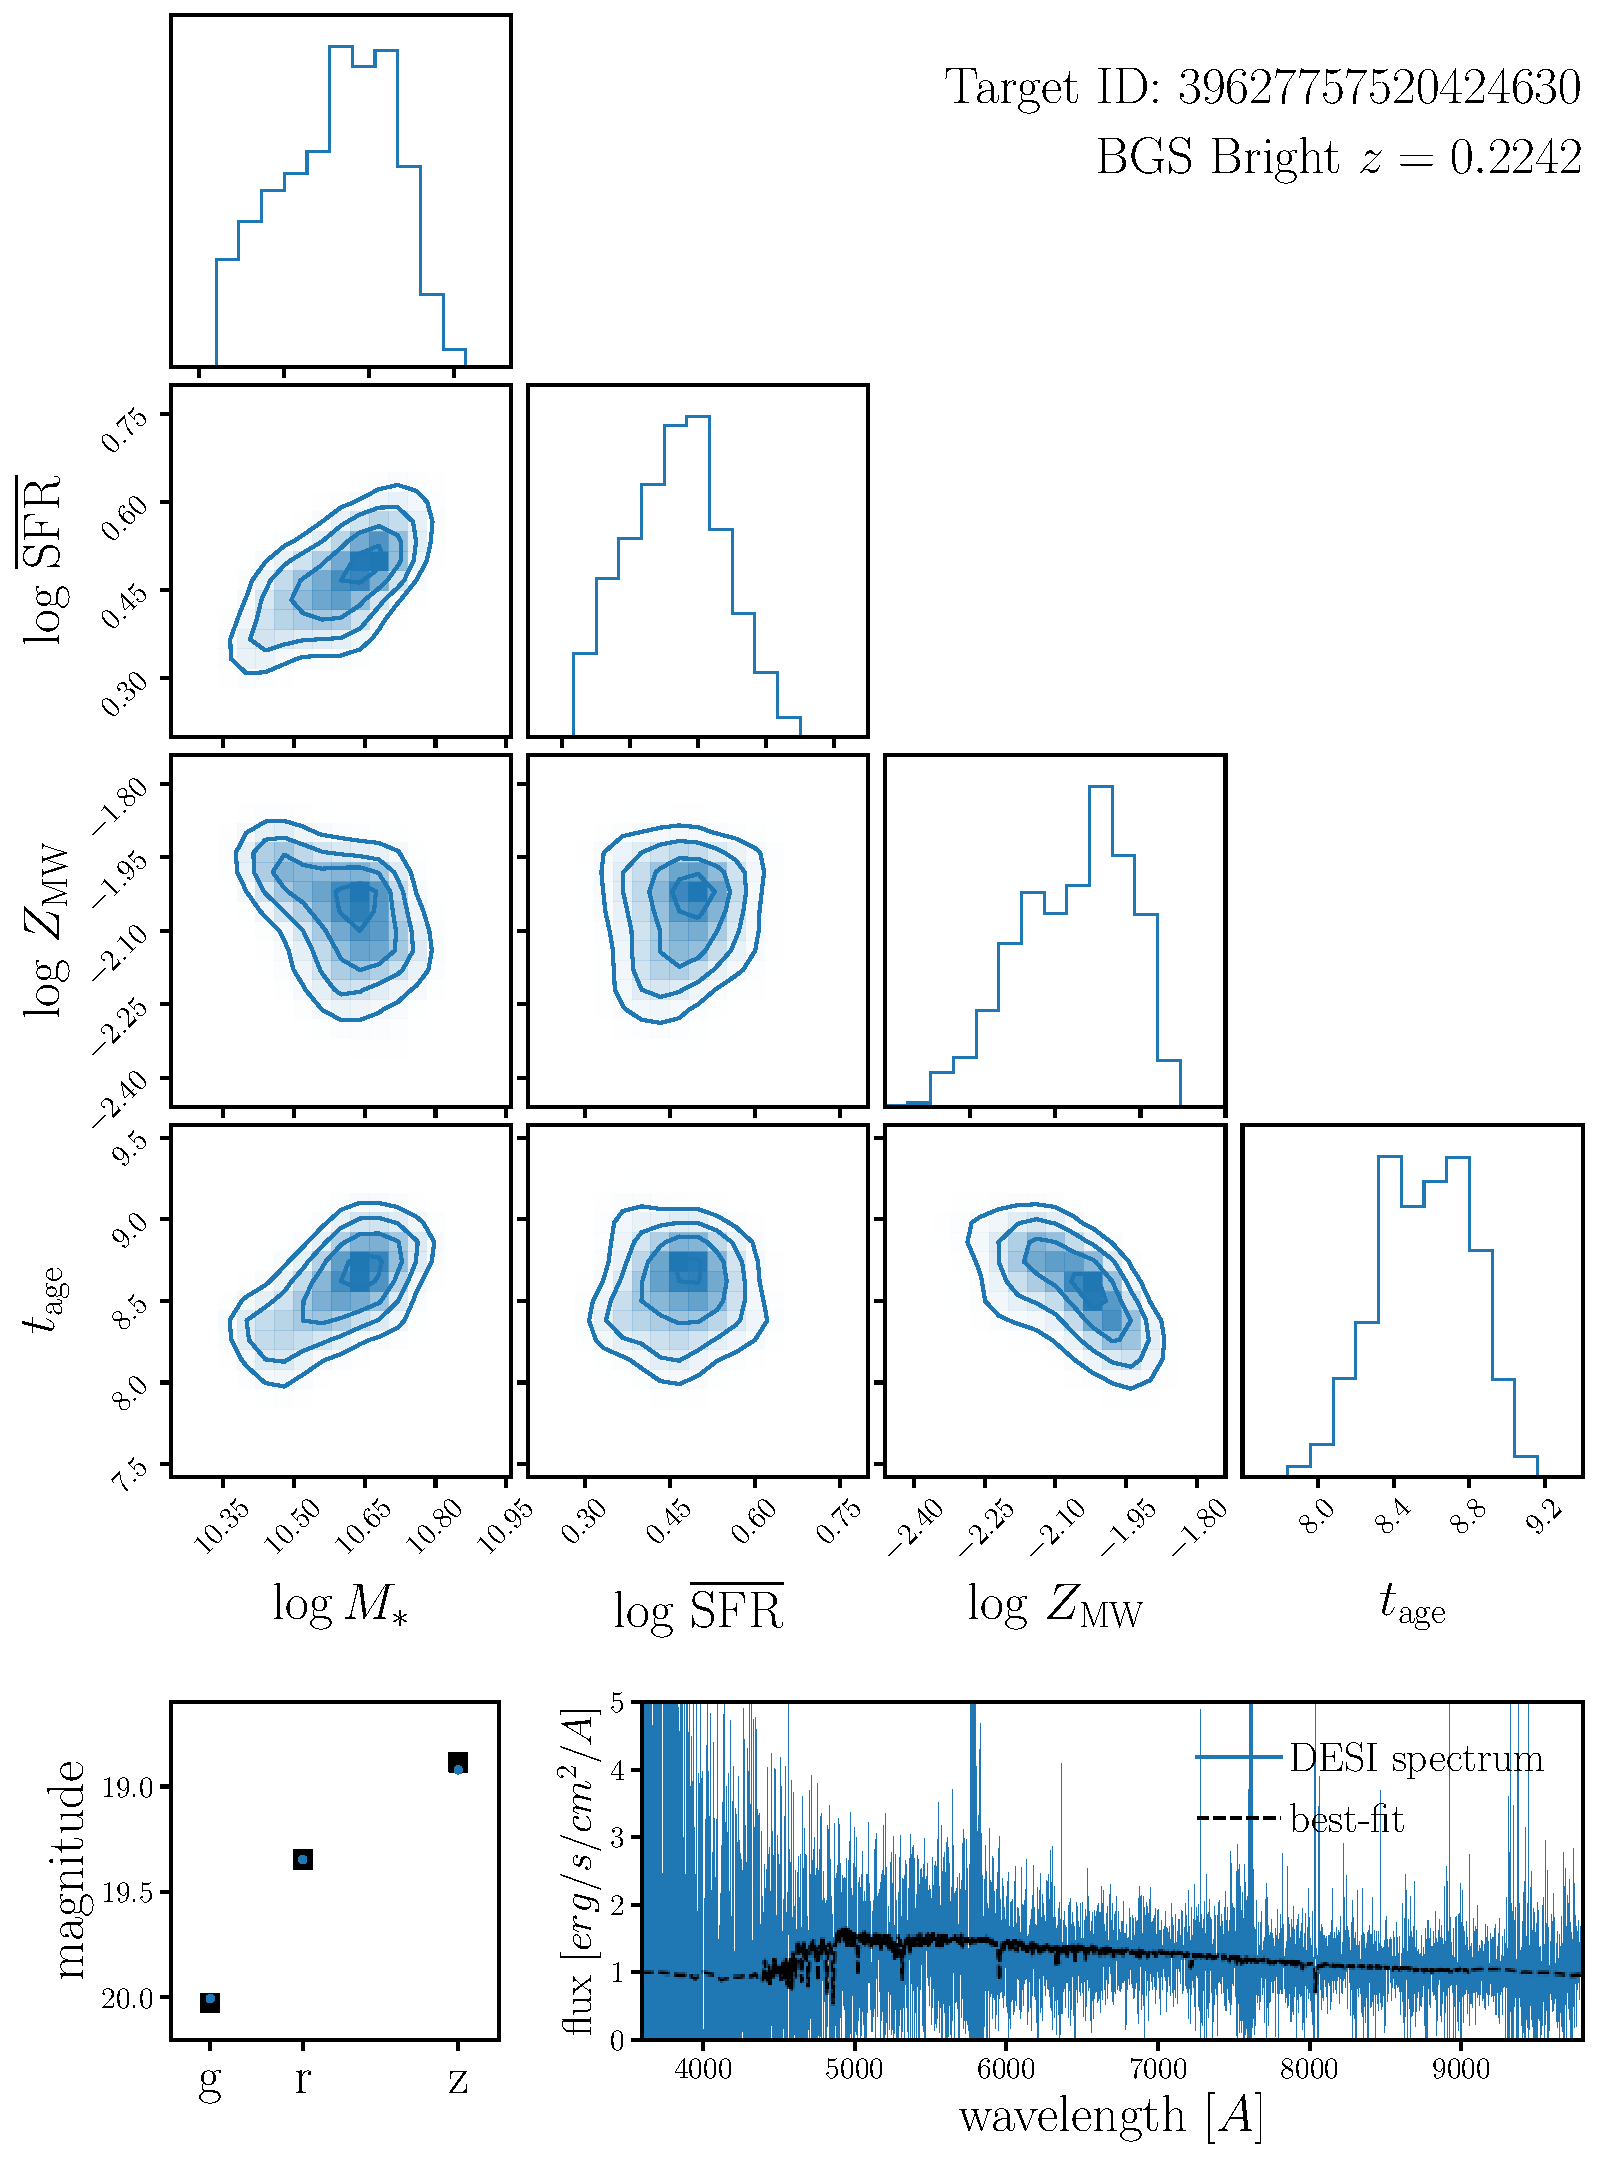
\includegraphics[width=0.6\textwidth]{figs/provabgs_posterior.pdf}
    \caption{
        {\em Top panels}: 
        Posteriors of galaxy properties, $M_*$, $\overline{\rm SFR}$, 
        $Z_{\rm MW}$, and $t_{\rm age, MW}$, for a randomly selected BGS 
        Bright galaxy with $z=0.2242$ (target ID: 39627757520424630) inferred
        using the PROVABGS SED modeling framework from DESI photometry and
        spectroscopy. 
        The contours mark the {\color{red} X, X, and X} percentiles of
        posterior. 
        With the PROVABGS posteriors, we accurately estimate the galaxy
        properties, their uncertainties, and any degeneracies among them. 
        {\em Bottom panels}: 
        Comparison of the best-fit PROVABGS SED model prediction (black) to
        observations (blue). 
        We compare the $g$, $r$, and $z$ band photometry in the left panel and 
        spectra in the right panel. 
        We infer the posterior of galaxy properties for every BGS galaxies in
        the DESI One-Percent Survey.
    }\label{fig:posterior}
\end{center}
\end{figure}


\begin{figure}
\begin{center}
    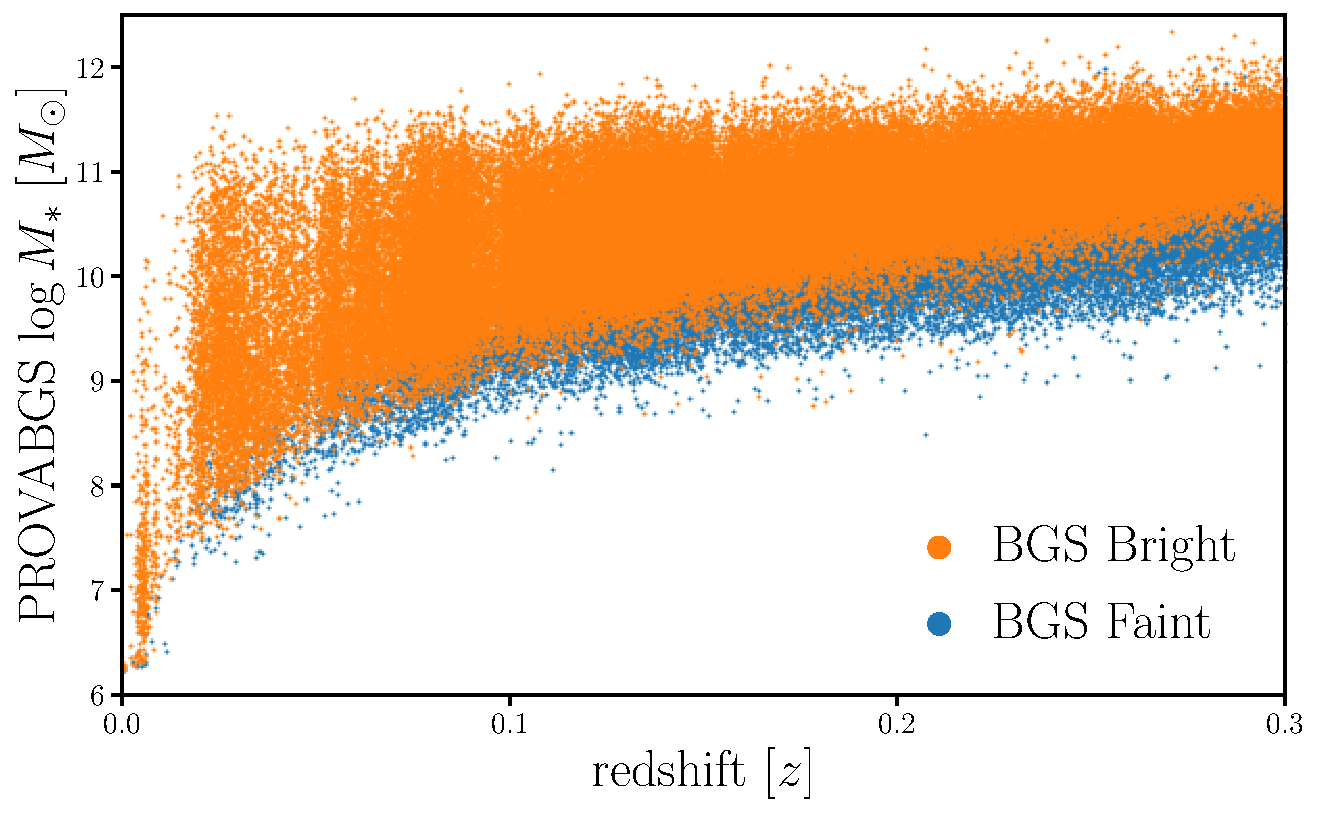
\includegraphics[width=0.6\textwidth]{figs/mstar_z.pdf}
    \caption{
        $M_*$ as a function of $z$ of BGS Bright (blue) and Faint (orange)
        galaxies in the DESI One-Percent Survey. 
        For $M_*$, we use the best-fit values derived using PROVABGS. 
        BGS Bright is a magnitude-limited sample to $r < 19.5$ while BGS Faint
        includes fainter galaxies $19.5 < r < 20.175$ selected using $r_{\rm
        fib}$ and color~\citep{hahn2022a}. 
        In total, we infer the posteriors of 143,017 BGS Bright and 95,499 BGS
        Faint galaxies in the DESI One-Percent Survey spanning $0 < z < 0.6$. 
    }\label{fig:mstar_z}
\end{center}
\end{figure}


In Figure~\ref{fig:posterior}, we demonstrate the PROVABGS SED modeling
framework for a randomly selected BGS Bright galaxy with $z=0.2242$ 
(target ID: 39627757520424630).
In the top panels, we present the posteriors of galaxy properties, $M_*$, 
$\overline{\rm SFR}$, $Z_{\rm MW}$, and $t_{\rm age, MW}$, inferred from DESI
photometry and spectroscopy. 
We mark the {\color{red} X, X, and X} percentiles of posterior with the
contours. 
The posteriors illustrate that we can precisely measure the properties of BGS
galaxies from DESI photometry and spectroscopy. 
Furthermore, with the full posterior, we accurately estimate the uncertainties
on the galaxy properties and the degeneracies among them (\emph{e.g.} $M_*$ and
$\overline{\rm SFR}$). 
In the bottom panels, we compare the PROVABGS SED model prediction using the
best-fit parameter values (black) to DESI observations (blue). 
The left panel compares the optical $g$, $r$, and $z$ band photometry while the
right panel compares the spectra. 
The comparison shows good agreement between the best-fit model and the
observations. 

We derive a PROVABGS posterior (\emph{e.g.} Figure~\ref{fig:posterior}) for
every galaxy in the DESI One-Percent Survey. 
In Figure~\ref{fig:mstar_z}, we present the best-fit $M_*$ measurements as a
function of $z$ for the BGS galaxies in DESI One-Percent Survey. 
We mark the galaxies in the BGS Bright sample in blue and the ones in the BGS
Faint sample in orange. 
We infer the posteriors of 143,017 BGS Bright and 95,499 BGS Faint galaxies. 
